\documentclass[10pt,a4paper]{article}
\usepackage[utf8]{inputenc}
\usepackage{amsmath}
\usepackage{amsfonts}
\usepackage{amssymb}
\usepackage{graphicx}
\usepackage[spanish]{babel}
\usepackage[utf8]{inputenc}
\usepackage{amssymb, amsmath}
\author{Angel Josue Loayza Huarachi}
\title{Lista de Ejercicios}
\graphicspath{ {c:/User/Angel/Pictures/Saved Pictures/} }

\usepackage{listings}

\begin{document}

\begin{titlepage}
	\centering
	{\bfseries\LARGE Universidad Catolica San Pablo \par}
	\vspace{1cm}
	{\scshape\Large Ciencias de la Computacion \par}
	\vspace{3cm}
	{\scshape\Huge Lista de Ejercicios \par}
	\vspace{3cm}
	{\Large Autor: \par}
	{\Large Angel Josue Loayza Huarachi \par}
	\vfill
	{\Large Mayo 2022 \par}
\end{titlepage}

\tableofcontents
\newpage

\section{Ejercicio 1}
	Utilizando las reglas de notacion asintoticas, demuestre las expresiones son verdaderas o falsas, justificando con la propia demostracion matematica y tambien con un breve comentario en caso sea necesario. Asuma que toda funcion presentada es positiva.
	\begin{itemize}
		\item 
			$max(f(n),g(n))=\theta(f(n)+g(n))$ \\
			\begin{equation*}
				 f(n) = max(f(n),g(n)) 
			\end{equation*}
			\begin{equation*}
				 g(n) = max(f(n),g(n))\\
			\end{equation*}
			Entonces
			\begin{equation*}
					C_{1}g(n) \leq  f(n) \leq C_{2}g(n)\\
			\end{equation*}
			\begin{equation*}
				C_{1}*(f(n)+g(n)) \leq  max(f(n),g(n)) \leq C_{2}*(f(n)+g(n)) 
			\end{equation*}
			\begin{enumerate}
				\item Sabemos que $f(n) + g(n) \leq max(f(n),g(n))$. \\Entonces: $max(f(n),g(n)) = O(f(n)+g(n))$
				\item Sabemos que $f(n) \leq f(n)+ g(n)$ y que $g(n) \leq f(n)+ g(n)$, pues sea cual sea el mayor entre f(n) o g(n), siempre seran menores a la suma de estos 2; por ello, cada uno de ellos tambien se considedra menor. \\Entonces: $max(f(n),g(n)) = \Omega (f(n)+g(n))$ (limite asintotico inferior)
			\end{enumerate}
			Pero, para ser verdad, $C_{1}$ debe ser $\geq  1$ para no volverla negativa o cero. Y $C_{2}$ debe ser $\geq  2$, para evitar volverlo negativo, cero, y definitivamente mayor a $C_{1}$\\
			Comentario:\\ El limite asintotico superior sera verdadero para todo $C_{1}\geq  1$.\\El limite asintotico inferior sera verdadero para todo $C_{2}\geq  2$.
		\item 
			$(n + a)^{b} = \Theta (n^{b}) | a, b \epsilon R^{+}, b > 0$
			\begin{equation*}
				 f(n) = (n + a)^{b} 
			\end{equation*}
			\begin{equation*}
				 g(n) = n^{b}
			\end{equation*}
			Entonces
			\begin{equation*}
					C_{1}g(n) \leq  f(n) \leq C_{2}g(n)\\
			\end{equation*}
			\begin{equation*}
				C_{1}*n^{b} \leq  (n + a)^{b} \leq C_{2}* n^{b} 
			\end{equation*}
			Delimitamos a:
			\begin{equation*}
				Si a = 0 
			\end{equation*}
			\begin{equation*}
				C_{1}*n^{b} = (n+0)^{b}
			\end{equation*}
			\begin{equation*}
				C_{1}*n^{b} = n^{b}
			\end{equation*}
			 El cual cumple para $C_{1} = 1$. Entonces $a \leq 0$ o $\left |a  \right |$\\
			 Tomar en cuenta:
			 \begin{itemize}
			 	\item Si $\left |a  \right | \leq n $. Entonces $ n + a \leq n + \left |a  \right | \leq 2n$. Pues como n es mator que "a", su valor absoluto sera mayor o igual. Y de igual forma, el doble de n, siempre sera mayor que la suma de estos. \\
			 	\item Si $\left |a  \right | \leq \frac{1}{2} $. Entonces $ n + a \geq  n - \left |a  \right | \geq  \frac{1}{2}n$. Pues como n es mayor que -a-, su valor absoluto sera mayor o igual. Y de igual forma, el doble de n, siempre sera mayor que la suma de estos. \\
			 \end{itemize}
			 
			 Entonces tenemos:
			 \begin{itemize}
			 	\item Inecuaciones: 
			 		\begin{equation*}
						n+a \leq n+\left |a  \right | \leq 2n
					\end{equation*}
					\begin{equation*}
						n + a \geq  n - \left |a  \right | \geq  \frac{1}{2}n
					\end{equation*}
					Entonces: 
					\begin{equation*}
						\frac{1}{2}n \leq n + a \leq 2n
					\end{equation*}
					\begin{equation*}
						(\frac{1}{2}n)^{b} \leq (n + a)^{b} \leq (2n)^{b}
					\end{equation*}
					\begin{equation*}
						(\frac{1}{2})^{b}(n)^{b} \leq (n + a)^{b} \leq (2)^{b}(n)^{b}
					\end{equation*}
			 	\item Condicionales: 
			 		\begin{equation*}
						Si \left |a  \right | \leq n
					\end{equation*}
			 		\begin{equation*}
						Si \left |a  \right | \leq \frac{1}{2}n \rightarrow 2\left |a  \right | \leq n
					\end{equation*}
			 \end{itemize}
			 Comentario: \\
			 Para $C_{1} = (\frac{1}{2})^{b}$, $C_{2} = (2)^{b}$ y  $n_{0} = 2\left |a  \right |$, satisface la ecuacion.
			 
		\item $2^{n+1} = O(2^{n})$
			\begin{equation*}
				 f(n) = (2)^{n+1} 
			\end{equation*}
			\begin{equation*}
				 g(n) = 2^{n}
			\end{equation*}
			Entonces
			\begin{equation*}
				f(n) \leq C g(n)
			\end{equation*}
			\begin{equation*}
				(2)^{n+1}  \leq C 2^{n}
			\end{equation*}
			\begin{equation*}
				\frac{(2)^{n+1}}{2^{n}} \leq \frac{C 2^{n}}{2^{n}} 
			\end{equation*}
			\begin{equation*}
				\frac{(2)^{n+1}}{2^{n}} \leq C 
			\end{equation*}
			\begin{equation*}
				(2)^{(n+1)-n}\leq C 
			\end{equation*}
			\begin{equation*}
				(2)^{1}\leq C 
			\end{equation*}
			\begin{equation*}
				2\leq C 
			\end{equation*}
			Tomamos valores C = 3 y n = 0:
			\begin{equation*}
				(2)^{n+1}  \leq C 2^{n}
			\end{equation*}
			\begin{equation*}
				(2)^{1}  \leq 3*2^{0}
			\end{equation*}
			\begin{equation*}
				2 \leq 3 \rightarrow Verdad
			\end{equation*}
			Comentario: \\
			Satisface la ecuacion cuando $C = 3$ y $n_{0} = 0$, $\forall n \geq n_{0}$
		\item $2^{2n} = O(2^{n})$
			\begin{equation*}
				 f(n) = (2)^{2n} 
			\end{equation*}
			\begin{equation*}
				 g(n) = 2^{n}
			\end{equation*}
			Entonces
			\begin{equation*}
				f(n) \leq C g(n)
			\end{equation*}
			\begin{equation*}
				(2)^{2n}  \leq C 2^{n}
			\end{equation*}
			\begin{equation*}
				\frac{(2)^{2n}}{2^{n}} \leq C 
			\end{equation*}
			\begin{equation*}
				2^{2n-n}\leq C 
			\end{equation*}
			\begin{equation*}
				2^{n}\leq C 
			\end{equation*}
			Tomamos valores n = 1:
			\begin{equation*}
				2^{n}  \leq C
			\end{equation*}
			\begin{equation*}
				2 \leq C
			\end{equation*}
			Tomamos valores n = 2:
			\begin{equation*}
				2^{2}  \leq C
			\end{equation*}
			\begin{equation*}
				4 \leq C
			\end{equation*}
			Tomamos valores n = 3:
			\begin{equation*}
				2^{3}  \leq C
			\end{equation*}
			\begin{equation*}
				8 \leq C
			\end{equation*}
			Comentario: \\
			Nunca una constante sera mayor a una funcion exponencial, por lo que $2^{2n}$ no tendria un limite asintotico superior en $2^{2}$
					
		\item $ \log{2}\log_{2}{n} =  O(\log{\log{n}})$ 
		
		
		\item Probar por induccion \\
			\begin{equation*}
				\sum_{i=1}^{n} \frac{1}{i^{2}} \leq 2 - \frac{1}{n}
			\end{equation*}
			\begin{equation*}
				\frac{1}{1} + \frac{1}{4} + \frac{1}{9} + \frac{1}{16} + ... + \frac{1}{n^{2}} \leq    2 - \frac{1}{n}
			\end{equation*}
			\begin{enumerate}
				\item Paso Base: Probamos con cualquier numero\\
					\begin{equation*}
						P(n_{0}) = P(1)
					\end{equation*}
					\begin{equation*}
						n_{0} = 1
					\end{equation*}
					\begin{equation*}
						P(1) = 2 - \frac{1}{1}
					\end{equation*}
					\begin{equation*}
						P(1) = 2 - 1
					\end{equation*}
					\begin{equation*}
						P(1) = 1
					\end{equation*}
					La formula es verdadera para $n_{0}$					
				\item Paso inductivo: \\ 
					Si la formula es verdadera\\
					Entonces tambien es verdadera para n = k y para n = k+1. \\
					Entonces:
					\begin{equation*}
						P(k) = P(k+1)
					\end{equation*}
					Hipotesis Inductiva
					\begin{equation*}
						P(k) = \sum_{i=1}^{k} \frac{1}{i^{2}} \leq 2 - \frac{1}{k}
					\end{equation*}
					Tenemos que demostrar 
					\begin{equation*}
						P(k+1) = \sum_{i=1}^{k+1} \frac{1}{i^{2}} \leq 2 - \frac{1}{k+1}
					\end{equation*}
					\begin{equation*}
						\sum_{i=1}^{k+1} = \sum_{i=1}^{k} \frac{1}{i^{2}} + \frac{1}{k+1}
					\end{equation*}
					\begin{equation*}
						 = 2- \frac{1}{n} + \frac{1}{k+1}
					\end{equation*}
					\begin{equation*}
						 = \frac{2n - 1}{n} + \frac{1}{k+1}
					\end{equation*}
					\begin{equation*}
						 = \frac{(2n-1)(k+1)+n}{n(k+1)}
					\end{equation*}
					\begin{equation*}
						 = \frac{(2nk+3n-k-1)}{n(k+1)}
					\end{equation*}
					Comentario: Por lo tanto no fue posible derivar la conclusion de la hipotesis. Esto significa que el predicado original es falso
			\end{enumerate}
			
		\item Probar por induccion
			\begin{equation*}
				[\frac{n}{2}]\left\{\begin{matrix}
				\frac{n}{2} \textup{, si n es par}\\ 
 				\frac{n+1}{2} \textup{, si n es impar}
				\end{matrix}\right.
			\end{equation*}
			\begin{enumerate}
				\item Paso Base (a) - Cuando n es par
					\begin{equation*}
						P(n_{0}) = P(2)
					\end{equation*}
					\begin{equation*}
						n_{0} = 2
					\end{equation*}
					\begin{equation*}
						P(2) = \frac{2}{2}
					\end{equation*}
					\begin{equation*}
						P(2) = 1  \textup{ La formula es verdadera para } n_{0}
					\end{equation*}
				\item Paso Inductivo (a)  - Cuando n es par\\
					Si la formula es verdadera\\
					Entonces tambien es verdadera para n = k y para n = k+1. \\
					Entonces:
					\begin{equation*}
						P(k) = P(k+1)
					\end{equation*}
					Hipotesis Inductiva:
					\begin{equation*}
						P(k) = \frac{k}{2} = \frac{k}{2}
					\end{equation*}
					Tenemos que demostrar 
					\begin{equation*}
						P(k+1) = \frac{k+1}{2} = \frac{k+1}{2}
					\end{equation*}
					\begin{equation*}
						\frac{k+1}{2} = \frac{k+1}{2}
					\end{equation*}
					\begin{equation*}
						k = k \textup{, Si es verdad para un n par}
					\end{equation*}
					
				\item Paso Base (b) - Cuando n es impar
					\begin{equation*}
						P(n_{0}) = P(1)
					\end{equation*}
					\begin{equation*}
						n_{0} = 1
					\end{equation*}
					\begin{equation*}
						P(1) = \frac{1+1}{2}
					\end{equation*}
					\begin{equation*}
						P(1) = 1
					\end{equation*}
				\item Paso Inductivo (b)  - Cuando n es impar\\
					Si la formula es verdadera\\
					Entonces tambien es verdadera para n = k y para n = k+1. \\
					Entonces:
					\begin{equation*}
						P(k) = P(k+1)
					\end{equation*}
					Hipotesis Inductiva:
					\begin{equation*}
						P(k) = \frac{k}{2} = \frac{k+1}{2}
					\end{equation*}
					Tenemos que demostrar 
					\begin{equation*}
						P(k+1) = \frac{k+1}{2} = \frac{(k+1)+1}{2}
					\end{equation*}
					\begin{equation*}
						\frac{k+1}{2} = \frac{k+2}{2}
					\end{equation*}
					\begin{equation*}
						2 \neq  4 \textup{, No es verdad para un n impar}
					\end{equation*}
			\end{enumerate}
		\item Probar por induccion 
			\begin{equation*}
				\forall n \geq 0, n^{5}-n \textup{ es divisible por 5}
			\end{equation*}
			\begin{enumerate}
				\item Paso Base
					\begin{equation*}
						P(n_{0}) = P(1)
					\end{equation*}
					\begin{equation*}
						n_{0} = 1
					\end{equation*}
					\begin{equation*}
						P(1) = 1^{5}-1
					\end{equation*}
					\begin{equation*}
						P(1) = 0 \textup{ La formula es verdad para } n_{0}
					\end{equation*}
				\item Paso Inductivo \\
					Asimilamos que es verdad\\
					Tiene que ser verdadera para n = k+1. \\
					Entonces:
					\begin{equation*}
						P(k) = P(k+1)
					\end{equation*}
					Hipotesis Inductiva:
					\begin{equation*}
						P(k) = k^{5}-k \textup{ es divisible por 5}
					\end{equation*}
					Demostramos
					\begin{equation*}
						P(k+1) = (k+1)^{5}-k - k +1
					\end{equation*}
					\begin{equation*}
						= k^{5}+(5k)^{4}+(10k)^{3}+(10k)^{2}+ 5k +1 - k +1
					\end{equation*}
					\begin{equation*}
						= k^{5}+(5k)^{4}+(10k)^{3}+(10k)^{2}+ 4k + 2
					\end{equation*}
					\begin{equation*}
						= k^{5}+5((k)^{4}+(2k)^{3}+(2k)^{2})+ 4k + 2
					\end{equation*}
					\begin{equation*}
						\textup{Como multiplica por 5, entonces si es divisible por 5}
					\end{equation*}
			\end{enumerate}
	\end{itemize}
	
\section{Ejercicio 2}
	La recurrencia $T(n) = 7T( \frac{n}{2} )+n^{2}$ representa la funcion de complejidad del algoritmo A. Un algoritmo alternativo A’ para el mismo problema tiene la siguiente ecuacion ${T}'(n) = a{T}'( \frac{n}{4} ) + n^{2}$. Cual es el
mayor numero entero a, que hace que el algoritmo A’ sea asintoticamente mas rapido que A.
	\begin{itemize}
		\item Caso de T(n) $= 7T \frac{n}{2}+n^{2}$
			\begin{equation*}
				T(n) = 7T \frac{n}{2}+n^{2} \rightarrow T(\frac{n}{2})
			\end{equation*}
			\begin{equation*}
				T(n) = 7(7T(\frac{\frac{n}{2}}{2})+ (\frac{n}{2})^{2})+n^{2}
			\end{equation*}
			\begin{equation*}
				T(n) = 7^{2}T(\frac{n}{2^{2}})+7(\frac{n}{2})^{2})+n^{2} \rightarrow T(\frac{n}{2^{2}})
			\end{equation*}
			\begin{equation*}
				T(n) = 7^{2}(7T(\frac{\frac{n}{2^{2}}}{2})+(\frac{n}{2^{2}})^{2})+7(\frac{n}{2})^{2})+n^{2} 
			\end{equation*}
			\begin{equation*}
				T(n) = 7^{3}T(\frac{n}{2^{3}})+7^{2}(\frac{n}{2^{2}})^{2}+7(\frac{n}{2})^{2}+n^{2} 
			\end{equation*}
			Entonces:
			\begin{equation*}
				T(n)<T(\frac{n}{2^{i-1}})> = 7^{i}T(\frac{n}{2^{i}})+7^{i-1}(\frac{n}{2^{i-1}})^{2}+ ... + 7(\frac{n}{2})^{2}+n^{2} 
			\end{equation*}
		\item Caso de T'(n) $ = aT'(\frac{n}{4})+n^{2}$
			\begin{equation*}
				T'(n) = aT'(\frac{n}{4})+n^{2} \rightarrow T'(\frac{n}{4})
			\end{equation*}
			\begin{equation*}
				T'(n) = a(aT'(\frac{\frac{n}{4}}{4})+ (\frac{n}{4})^{2})+n^{2}
			\end{equation*}
			\begin{equation*}
				T'(n) = a^{2}T'(\frac{n}{4^{2}})+a(\frac{n}{4})^{2})+n^{2} \rightarrow T(\frac{n}{4^{2}})
			\end{equation*}
			\begin{equation*}
				T'(n) = a^{2}(aT'(\frac{\frac{n}{4^{2}}}{4})+(\frac{n}{4^{4}})^{2})+a(\frac{n}{4})^{2}+n^{2} 
			\end{equation*}
			\begin{equation*}
				T'(n) = a^{3}T'(\frac{n}{4^{3}})+a^{2}(\frac{n}{4^{2}})^{2}+a(\frac{n}{4})^{2}+n^{2} 
			\end{equation*}
			Entonces:
			\begin{equation*}
				T'(n)<T'(\frac{n}{4^{i-1}})> = a^{i}T(\frac{n}{4^{i}})+a^{i-1}(\frac{n}{4^{i-1}})^{2}+ ... + a(\frac{n}{4})^{2}+n^{2} 
			\end{equation*}
	\end{itemize}
	Comentario: El valor del entero --a-- para que el algoritmo A' sea asintoticamente mas rapido que A es, el mismo al cuadrado $(a^{2})$, pues::
	\begin{equation*}
		A = 7^{i}T(\frac{n}{2^{i}})+... 
	\end{equation*}
	\begin{equation*}
		A' = a^{i}T(\frac{n}{4^{i}})+ ... \rightarrow a^{i}T(\frac{n}{(2^{2})^{i}})+ ... 
	\end{equation*}
\section{Ejercicio 3}
	Dada las siguientes ecuaciones de recurrencia, resolver utilizando expansion de recurrencia y teorema maestro. En ambos casos colocar todo el desarrollo no obviar partes. Si en caso no se pueda aplicar el teorema maestro, explique el motivo. Asuma que T(n) es constante para $n < 2$.
	\begin{itemize}
		\item $T(n) = 4T(\frac{n}{2})+n$
			\begin{equation*}
				a = 4
			\end{equation*}
			\begin{equation*}
				b = 2
			\end{equation*}
			\begin{equation*}
				f(n) = n
			\end{equation*}
			De tal forma que :
			\begin{equation*}
				n^{\log_{b}{a}} = n^{\log_{2}{4}} = n^{2}
			\end{equation*}
			Caso 1 Teorema Maestro
			\begin{equation*}
				f(n) = O(n^{\log_{b}{a}-\varepsilon})
			\end{equation*}
			\begin{equation*}
				n = O(n^{2-\varepsilon}) \textup{, para e = 1}
			\end{equation*}
			\begin{equation*}
				n = O(n)
			\end{equation*}
			Entonces:
			\begin{equation*}
				T(n) = O(n^{2})
			\end{equation*}
			
		\item $T(n) = 4T(\frac{n}{2})+n^{2}$
			\begin{equation*}
				a = 4
			\end{equation*}
			\begin{equation*}
				b = 2
			\end{equation*}
			\begin{equation*}
				f(n) = n^{2}
			\end{equation*}
			De tal forma que :
			\begin{equation*}
				n^{\log_{b}{a}} = n^{\log_{2}{4}} = n^{2}
			\end{equation*}
			Caso 2 Teorema Maestro
			\begin{equation*}
				f(n) = \Theta (n^{\log_{b}{a}})
			\end{equation*}
			\begin{equation*}
				n^{2} = \Theta (n^{2})
			\end{equation*}
			Entonces:
			\begin{equation*}
				T(n) = \Theta(n^{\log_{b}{a}}*\log{n})
			\end{equation*}
			\begin{equation*}
				T(n) = \Theta(n^{2}*\log{n})
			\end{equation*}
			
		\item $T(n) = 4T(\frac{n}{2})+n^{3}$
			\begin{equation*}
				a = 4
			\end{equation*}
			\begin{equation*}
				b = 2
			\end{equation*}
			\begin{equation*}
				f(n) = n^{3}
			\end{equation*}
			De tal forma que :
			\begin{equation*}
				n^{\log_{b}{a}} = n^{\log_{2}{4}} = n^{2}
			\end{equation*}
			Caso 3 Teorema Maestro
			\begin{equation*}
				af(\frac{n}{b}) < c f(n)
			\end{equation*}
			\begin{equation*}
				4(\frac{n}{2})^{3} < c f(n)
			\end{equation*}
			\begin{equation*}
				2n^{3} < cn^{3}
			\end{equation*}
			\begin{equation*}
				2 < c \textup{, Por lo que C = 3 cumple}
			\end{equation*}
			Entonces:
			\begin{equation*}
				F(n) = \Omega (n^{\log_{b}{a}+\varepsilon})  \textup{, para e = 1}
			\end{equation*}
			\begin{equation*}
				T(n) = \Theta(n^{3})
			\end{equation*}
			
		\item $T(n) = 4T(\frac{9n}{10})+n$
			\begin{equation*}
				a = 1
			\end{equation*}
			\begin{equation*}
				b = 10/9
			\end{equation*}
			\begin{equation*}
				f(n) = n
			\end{equation*}
			De tal forma que :
			\begin{equation*}
				n^{\log_{b}{a}} = n^{\log_{10/9}{1}} = n^{0} = 1
			\end{equation*}
			Caso 3 Teorema Maestro
			\begin{equation*}
				af(\frac{n}{b}) < c f(n)
			\end{equation*}
			\begin{equation*}
				1(\frac{9n}{10}) < cn
			\end{equation*}
			\begin{equation*}
				\frac{9n}{10} < cn
			\end{equation*}
			\begin{equation*}
				\frac{9}{10} < c \textup{, Por lo que C = 1 cumple}
			\end{equation*}
			Entonces:
			\begin{equation*}
				F(n) = \Omega (n^{\log_{b}{a}+\varepsilon})  \textup{, para e = 1}
			\end{equation*}
			\begin{equation*}
				T(n) = \Theta(n)
			\end{equation*}
			
		\item $T(n) = 16T(\frac{n}{4})+n^{2}$
			\begin{equation*}
				a = 16
			\end{equation*}
			\begin{equation*}
				b = 4
			\end{equation*}
			\begin{equation*}
				f(n) = n^{2}
			\end{equation*}
			De tal forma que :
			\begin{equation*}
				n^{\log_{b}{a}} = n^{\log_{4}{16}} = n^{\sqrt[1]{2}} = \sqrt{n}
			\end{equation*}
			Caso 3 Teorema Maestro
			\begin{equation*}
				af(\frac{n}{b}) < c f(n)
			\end{equation*}
			\begin{equation*}
				16(\frac{n}{4}) < cn^{2}
			\end{equation*}
			\begin{equation*}
				c = 2 \textup {, cumple}
			\end{equation*}
			Entonces:
			\begin{equation*}
				F(n) = \Omega (n^{\log_{b}{a}+\varepsilon})  \textup{, para e = 1}
			\end{equation*}
			\begin{equation*}
				T(n) = \Theta(n^{2})
			\end{equation*}
		\item $T(n) = 7T(\frac{n}{3})+n^{2}$
			\begin{equation*}
				a = 7
			\end{equation*}
			\begin{equation*}
				b = 3
			\end{equation*}
			\begin{equation*}
				f(n) = n^{2}
			\end{equation*}
			De tal forma que :
			\begin{equation*}
				n^{\log_{b}{a}} = n^{\log_{3}{7}} = n^{1.777}
			\end{equation*}
			Caso 3 Teorema Maestro
			\begin{equation*}
				af(\frac{n}{b}) < c f(n)
			\end{equation*}
			\begin{equation*}
				7(\frac{n}{3}) < cn^{2}
			\end{equation*}
			\begin{equation*}
				c = 1 \textup {, no cumple}
			\end{equation*}
			\begin{equation*}
				c = 2 \textup {, si cumple}
			\end{equation*}
			Entonces:
			\begin{equation*}
				F(n) = \Omega (n^{\log_{b}{a}+\varepsilon})  \textup{, para e = 0.222}
			\end{equation*}
			\begin{equation*}
				T(n) = \Theta(n^{2})
			\end{equation*}
		\item $T(n) = 2T(\frac{n}{4})+\sqrt{n}$
			\begin{equation*}
				a = 2
			\end{equation*}
			\begin{equation*}
				b = 4
			\end{equation*}
			\begin{equation*}
				f(n) = \sqrt{n}
			\end{equation*}
			De tal forma que :
			\begin{equation*}
				n^{\log_{b}{a}} = n^{\log_{4}{2}} = n^{\frac{1}{2}} = \sqrt{n}
			\end{equation*}
			Caso 2 Teorema Maestro
			\begin{equation*}
				f(n) = \Theta (n^{\log_{2}{4}})
			\end{equation*}
			\begin{equation*}
				\sqrt{n} = \Theta (\sqrt{n})
			\end{equation*}
			Entonces:
			\begin{equation*}
				T(n) = \Theta(n^{\log_{2}{4}}*\log{n})
			\end{equation*}
			\begin{equation*}
				T(n) = \Theta(\sqrt{n}*\log{n})
			\end{equation*}
			
		\item $T(n) = 4T(\frac{n}{2})+n^{2}\log{n}$
			\begin{equation*}
				a = 4
			\end{equation*}
			\begin{equation*}
				b = 2
			\end{equation*}
			\begin{equation*}
				f(n) = n^{2}*\log{n}
			\end{equation*}
			De tal forma que :
			\begin{equation*}
				n^{\log_{b}{a}} = n^{\log_{2}{4}} = n^{2}
			\end{equation*}
			Caso 1 Teorema Maestro
			\begin{equation*}
				f(n) = O(n^{\log_{b}{a}-\varepsilon})
			\end{equation*}
			\begin{equation*}
				n^{2}*\log{n} = O(n^{2-\varepsilon})\textup{, para e } \approx 1
			\end{equation*}
			Entonces:
			\begin{equation*}
				T(n) = O(n^{2}*\log{n})
			\end{equation*}
			
		\item $T(n) = T(n-1) + n$
			\begin{equation*}
				T(n) = T(n-1) + n \rightarrow T(n-1)
			\end{equation*}
			\begin{equation*}
				T(n) = (T(n-2)+n)+n
			\end{equation*}
			\begin{equation*}
				T(n) = T(n-2)+2n \rightarrow T(n-2)
			\end{equation*}
			\begin{equation*}
				T(n) = (T(n-3)+n)+2n
			\end{equation*}
			\begin{equation*}
				T(n) = T(n-3)+3n \rightarrow T(n-3)
			\end{equation*}
			\begin{equation*}
				...
			\end{equation*}
			\begin{equation*}
				T(n) = T(n-(n-1))+(n-1)n
			\end{equation*}
			\begin{equation*}
				T(n) = T(1)+n^{2}-n
			\end{equation*}
			\begin{equation*}
				T(n) = C +n^{2}-n
			\end{equation*}
			\begin{equation*}
				T(n) = O(O(c)+O(n^{2}))+(-n)
			\end{equation*}
			\begin{equation*}
				T(n) = O(c+n^{2}+n)
			\end{equation*}
			\begin{equation*}
				T(n) = O(n^{2})
			\end{equation*}
			
		\item $T(n) = \sqrt{n} + 1$
			\begin{equation*}
				T(n) = n^{\frac{1}{2}} + n
			\end{equation*}
			\begin{equation*}
				T(n) = O(O(n^{\frac{1}{2}})+O(n))
			\end{equation*}
			\begin{equation*}
				T(n) = O(n^{\frac{1}{2}}+n)
			\end{equation*}
			\begin{equation*}
				T(n) = O(n)
			\end{equation*}
	\end{itemize}

\section{Ejercicio 4}
	Se sabe que, para resolver el problema de ordenacion de numeros, el algoritmo Mergesort posee una complejidad de $\theta(n \log{n})$ y el Insertion Sort $O(n^{2})$. Sin embargo, los factores constantes del algoritmo Insertion lo tornan mas veloz para vectores de tama˜no n peque˜nos. Por ende tiene sentido realizar
una combinacion de ambos, y utilizar el algoritmo de insercion cuando los problemas se tornen lo suficientemente peque˜nos. Considere la siguiente modificacion del Mergesort: $\frac{n}{k}$ sub listas de tama˜no k son ordenadas utilizando el algoritmo de insercion, y luego combinadas utilizando el mecanismo del
Mergesort (Merge), siendo k la variable a ser determinada.

	\begin{lstlisting}[language=C++, caption={InsertionSort.hpp}, label={lst:listing-cpp}, breaklines=true]
	
void insertionSort(int arr[], int n)
{
	int a;
	int aux;
	int j;
	for (a = 1; a < n; a++)
	{
		aux = arr[a];
		j = a - 1;
		while (j >= 0 and arr[j] > aux)
		{
			arr[j + 1] = arr[j];
			j--;
		}
		arr[j + 1] = aux;
	}
}	
	
	\end{lstlisting}
	
	\begin{lstlisting}[language=C++, caption={InsertionSort.hpp}, label={lst:listing-cpp}, breaklines=true]
	
void mergeSort(int* A, int n)
{
	//base
	if (n == 1)
	{
		return;
	}
	//recurisivo
	int centro = n / 2;
	int* aux1izq = new int[centro];
	int* aux2der = new int[n - centro];

	//recorremos la primera parte
	for (int i = 0; i < centro; i++)
	{
		aux1izq[i] = A[i];
	}
	//recorremos la otra parte
	for (int i = centro; i < n; i++)
	{
		aux2der[i-centro] = A[i];
	}
	mergeSort(aux1izq, centro); //evaluacion recursivamente la primera mitad
	mergeSort(aux2der, n - centro); //evaluacion recursiva de la segunda mitad
    mergeaux(A, aux1izq, centro, aux2der); //obtenido de la tarea "Algoritmos de ordenacion"
}
	
	\end{lstlisting}
\section{Ejercicio 5}
	
	Para los problemas presentados, cree un codigo en $C ++$, presente la complejidad del algoritmo del cual es instancia el codigo presentado [1pt]. Cada codigo debera estar en latex es decir deben utilizar la biblioteca listings a b. Adicionalmente, deberan correr y colocar screenshots del codigo corriendo con las instancias que se les pida por cada problema.

	\begin{itemize}

\item Desarrolle un programa “Recursivo” para generar la descomposici´on de un n´umero entero positivo, en la suma de todos los posibles factores. La presentaci´on de los factores debe estar ordenada de mayor a menor. Por ejemplo para n = 5
\begin{lstlisting} [language=C++, caption={DescompositionNumber.hpp - Sum decomposition algorithm}, label={lst:listing-cpp}, breaklines=true]

#include <iostream>
#include <vector>
#include <stdio.h>
#pragma once

using namespace std;

/* Example
5
4 1
3 2
3 1 1
2 2 1
2 1 1 1 
1 1 1 1 1
*/

void printVector(vector <int> v)
{
	for (auto i = v.begin(); i != v.end(); ++i)
		cout << *i << " ";
}

void printarr(int *A, int i)
{
	//for (int j = i; j < sizeof(A)/ sizeof(A[0]); j++)
	for (int j = i; j > 0; j--)
	//for (int j = 0; j < i; j++)
	{
		cout << A[j-1] << " ";
	}
	cout << endl;	
}

void descompositionNumber(int n, int i, int tam)
{
	static int* arr = new int[tam];
	if (n == 0)
	{ 
		printarr(arr, i);
	}

	if (n > 0)
	{
		int j;
		for (j = tam; j > 0; j--)
		{
			arr[i] = j;
			descompositionNumber(n - 1, i + 1, j);
		}
	}
}

\end{lstlisting}

\item Dado un vector con n numeros enteros, determine la maxima suma en un subvector contiguo de ese vector. Si todos los n´umeros fueran negativos asuma que la suma es 0.
\begin{lstlisting} [language=C++, caption={maxSum.hpp - Maximum sum in a vector}, label={lst:listing-cpp}, breaklines=true]

#include <iostream>
#pragma once

using namespace std;

int maxSum(int A[], int n)
{
	int aux1 = 0; 			//C
	int aux2 = 0;			//C

	int sum1 = 0;			//C
	int result = 0; // para la respuesta final //C
		
	//maxima suma entre todos los numeros
	for (int i = 0; i < n; i++)		//N
	{
		sum1 = sum1 + A[i];		//N
	}

	int aux3 = sum1;			//C
	int sum2 = sum1;			//C

	// COMPROBACION DE IZQUIERDA A DERECHA
	for (int i = 0; i < n; i++)		//N
	{
		//vamos restando a la suma total los elementos del vector	 
		aux3 = aux3 - A[i];		//N
		if (aux3 > sum1)		//N
		{
		 	//reemplazamos sum1 porque encontramos un numero mayor 
			sum1 = aux3;		//N
 			// marcamos donde encontramos un mayor			
			aux1 = i;		//N
		}
	}

	int aux4 = sum2;			//C
	
	// COMPROBACION DE DERECHA A IZQUIERDA				 
	for (int i = n - 1; i >= 0; i--)	//N
	{
		aux4 = aux4 - A[i];		//N
		if (aux4 > sum2)		//N
		{
			sum2 = aux4;		//N
			// marcamos donde encontramos un mayor	
			aux2 = i; 		//N
		}
	}

	for (int i = aux1 + 1; i <= aux2 - 1; i++)   //N
	{
		result = result + A[i];		 //N
	}

	return result;

}
/* Complejidad
O( 7 O(C) + 14 O(N) )
O( O(C) + O(N) )
O( O(N) )
complejidad de O(N) 
*/

\end{lstlisting}

\end{itemize}

\newpage
	\begin{figure}
		\caption{Sum decomposition algorithm and Maximum sum in a vector}
		\centering
		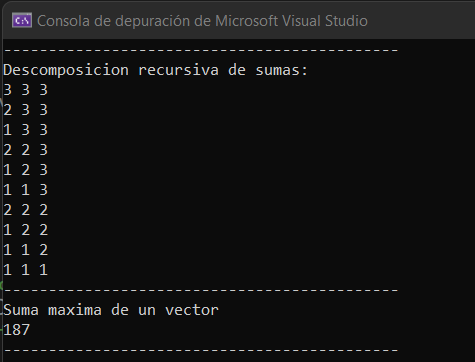
\includegraphics[scale=1.5]{ScrenshotCode}
	\end{figure}
	
\end{document}
